\documentclass{article}
\usepackage[submission]{colm2026_conference}

\usepackage{microtype}
\usepackage{hyperref}
\usepackage{url}
\usepackage{booktabs}
\usepackage{graphicx}
\usepackage{amsmath}
\usepackage{amssymb}
\usepackage{tabularx}
\usepackage{makecell}
\usepackage{subcaption}
\usepackage{enumitem}
\usepackage{placeins}
\usepackage{xcolor}
\usepackage{lineno}

\input{math_commands}
% Auto-generated by scripts/paper/build_colm2026_assets.py
\newcommand{\MergedRunId}{paper\_merged\_9x1000\_20260330T122258Z}
\newcommand{\PreparedExampleCount}{1000}
\newcommand{\ScoreRowCount}{54,000}
\newcommand{\MetricRowCount}{54,000}
\newcommand{\TokenAuditCount}{258,876}
\newcommand{\SemanticIdentityValidCases}{7,301}
\newcommand{\PooledLagMedian}{19.2}
\newcommand{\PooledLagCILow}{18.9}
\newcommand{\PooledLagCIHigh}{19.5}
\newcommand{\FlagshipTwentyPlausiblePct}{72\%}
\newcommand{\FlagshipTwentyCommittedPct}{4\%}
\newcommand{\FlagshipFiftyPlausiblePct}{86\%}
\newcommand{\FlagshipFiftyCommittedPct}{9\%}
\newcommand{\FlagshipEightyPlausiblePct}{94\%}
\newcommand{\FlagshipEightyCommittedPct}{30\%}
\newcommand{\ArcPromptCount}{195}
\newcommand{\CsqaPromptCount}{794}
\newcommand{\MmluPromptCount}{11}
\newcommand{\OverallPrimaryPositiveCells}{21}
\newcommand{\OverallPrimaryEvaluableCells}{21}
\newcommand{\OverallPrimaryInsufficientCells}{6}
\newcommand{\OverallSecondaryPositiveCells}{21}
\newcommand{\OverallSecondaryEvaluableCells}{21}
\newcommand{\OverallSecondaryInsufficientCells}{6}
\newcommand{\ArcCsqaPositiveCells}{18}
\newcommand{\ArcCsqaEvaluableCells}{18}
\newcommand{\MmluPositiveCells}{3}
\newcommand{\MmluEvaluableCells}{3}
\newcommand{\MmluInsufficientCells}{6}
\newcommand{\GoldArcCsqaPositiveCells}{18}
\newcommand{\GoldArcCsqaEvaluableCells}{18}
\newcommand{\GoldMmluInsufficientCells}{9}
\newcommand{\SemanticIdentityValidRate}{81\%}
\newcommand{\TemplatedIdentityValidRate}{58\%}
\newcommand{\LetterIdentityValidRate}{95\%}
\newcommand{\TemplatedAgreementIdentity}{60\%}
\newcommand{\LetterAgreementIdentity}{44\%}
\newcommand{\AllSameReadoutRate}{31\%}
\newcommand{\DuplicateOptionCount}{17}
\newcommand{\TokenCollisionCount}{1224}


\graphicspath{{figures/}}

\definecolor{darkblue}{rgb}{0, 0, 0.5}
\hypersetup{colorlinks=true, citecolor=darkblue, linkcolor=darkblue, urlcolor=darkblue}

\title{When Models Commit: Candidate Formation and Winner Isolation Across Model Depth}
\author{Anonymous Authors}

\begin{document}

\ifcolmsubmission
\linenumbers
\fi

\maketitle

\begin{abstract}
Language models produce one final answer, but the forward pass may involve two stages before that answer appears: the model may first narrow the set of answers that still look possible, and only later commit to one winner. We study that gap in multiple-choice question answering.

For each prompt, we end the rendered question with the literal suffix \texttt{"Final answer: "} and score exact continuations layer by layer. On the primary path, the continuation is the option text itself. This lets us track when the eventual answer first enters a small plausible-answer set, when it becomes the stable top prediction, and when it opens a persistent margin over the runner-up. We run the analysis on nine instruction-tuned open-weight models from the Qwen, Gemma, and Llama families on a 1{,}000-example slice of ARC-Challenge, CommonsenseQA, and the full 11-question MMLU abstract-algebra validation slice.

The main pattern is clear. In the pooled primary analysis, by 20\% of normalized depth the eventual answer is already in the plausible set for \FlagshipTwentyPlausiblePct{} of evaluable cases, but stable commitment has happened in only \FlagshipTwentyCommittedPct{}. All \ArcCsqaPositiveCells{} evaluable ARC-Challenge and CommonsenseQA model-dataset cells are positive under the preregistered primary rule. The \MmluPositiveCells{} evaluable MMLU cells are also positive, but that benchmark slice is mostly underpowered because it contains only \MmluPromptCount{} questions.

We also score two answer-format controls after the same prompt suffix: the literal continuation \texttt{"The answer is \{option\}"} and the answer letter alone. These controls often change both which cases are evaluable and which answer wins at the final layer, so they are useful checks on answer-format effects rather than replacements for exact option-text scoring. In the setting we study, models usually treat the eventual answer as a serious possibility well before they fully commit to it.
\end{abstract}

\section{Introduction}

A multiple-choice answer hides more than one decision. A model can first narrow the field to a few answers that still seem possible and only later settle on one final winner. Standard evaluation only shows the last step. It tells us what answer came out, but not when that answer first became a serious option inside the network.

This paper asks a simple question. Does the eventual answer become one of the plausible answers before the model writes the margin that finally separates it from the runner-up? Figure~\ref{fig:flagship} previews the answer. In the pooled primary analysis, by 20\% of normalized depth the eventual answer is already in the plausible answer set for \FlagshipTwentyPlausiblePct{} of evaluable cases, but only \FlagshipTwentyCommittedPct{} are already stably committed.

We answer that question in a very literal way. We build a normal multiple-choice prompt, end it with the suffix \texttt{"Final answer: "}, and then score the exact strings the model could write next. On the main path, that string is the full option text itself, such as \texttt{"photosynthesis"}. So instead of asking an external probe to guess the answer, we watch how the model's own answer strings rise and fall across depth.

Our setting is intentionally narrow and easy to audit. We evaluate nine instruction-tuned open-weight models from the Qwen 2.5 Instruct, Gemma 2 IT, and Llama Instruct families on a 1{,}000-example slice spanning ARC-Challenge, CommonsenseQA, and MMLU abstract algebra. The claim of the paper is limited to that setting. Within it, the pattern is consistent: the eventual answer usually enters the plausible answer set well before it becomes stably isolated from the runner-up. All \ArcCsqaPositiveCells{} evaluable ARC-Challenge and CommonsenseQA model-dataset cells are positive under the preregistered primary rule (Figure~\ref{fig:forest}, Table~\ref{tab:primary-summary}). The MMLU abstract-algebra slice is much smaller, so it is too small to carry much weight on its own.

The paper makes three contributions. First, it gives a simple measurement framework for separating ``still possible'' from ``finally chosen'' without leaving the answer strings that appear in the task itself. Second, it shows a large and consistent gap between those two stages in the pooled curves and in every evaluable ARC-Challenge and CommonsenseQA cell. Third, it shows that small changes to answer format, such as switching from full option text to an answer letter, can change both coverage and winners. That makes those alternatives useful controls, but not replacements for exact option-text scoring.

\begin{figure*}[t]
\centering
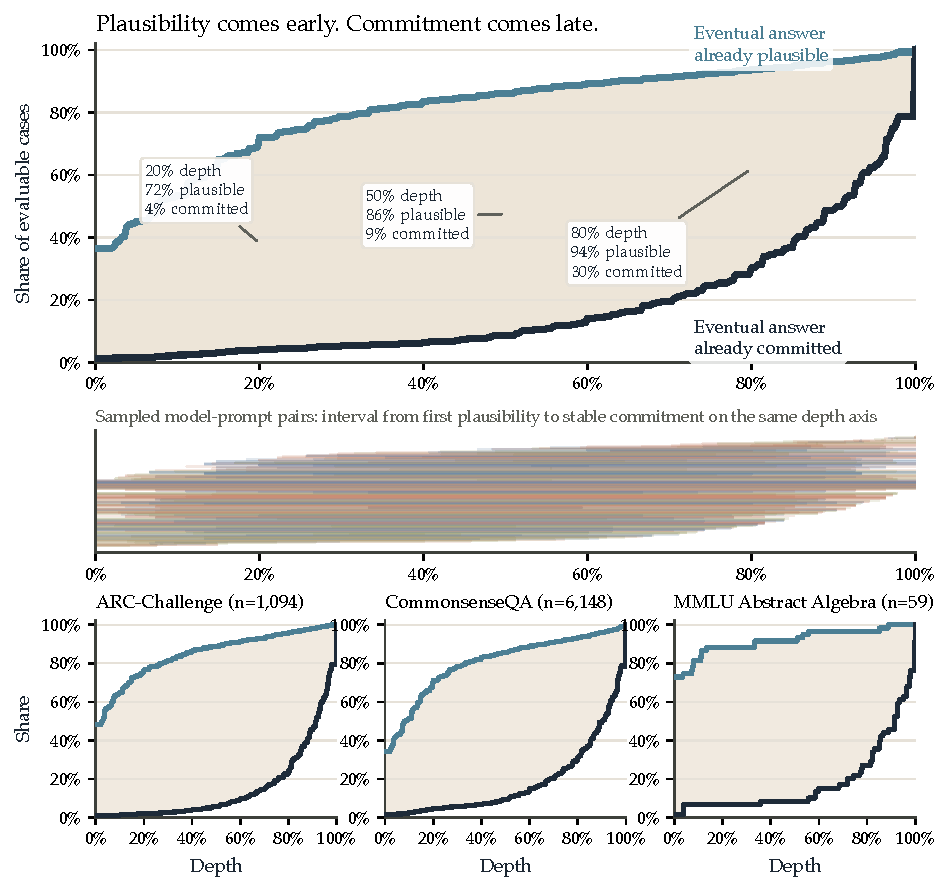
\includegraphics[width=\textwidth]{figure1_flagship_plausibility_commitment.pdf}
\caption{\textbf{The eventual answer becomes plausible much earlier than it becomes committed.} The top panel pools all evaluable model-prompt pairs from the primary analysis path (\texttt{semantic\_exact} with identity ordering). The light curve asks: by this depth, in how many cases is the eventual answer already one of the plausible answers? The dark curve asks: by this depth, in how many cases has the model already opened a stable winner-runner margin that it keeps through the end of the network? The band between the curves is the main object in the paper: cases where the answer already looks plausible but the model has not fully committed yet. The interval strip shows a sample of individual cases on the same normalized-depth axis, and the three bottom panels show the same pattern separately for ARC-Challenge, CommonsenseQA, and MMLU abstract algebra.}
\label{fig:flagship}
\end{figure*}

\section{Setup and measurement}

Table~\ref{tab:design-summary} summarizes the experiment design. The model panel contains nine instruction-tuned checkpoints from three families: Qwen 2.5 Instruct~\citep{qwen25card}, Gemma 2 IT~\citep{gemma2card}, and Llama Instruct~\citep{llama3herd}. The dataset slice contains \ArcPromptCount{} ARC-Challenge prompts~\citep{clark2018arc}, \CsqaPromptCount{} CommonsenseQA prompts~\citep{talmor2019commonsenseqa}, and the full \MmluPromptCount{}-question MMLU abstract-algebra validation slice~\citep{hendrycks2021mmlu}. The MMLU count is small because this benchmark slice itself is small in our setup; we did not drop a larger set of abstract-algebra questions.

For every model, we render a normal multiple-choice prompt and end it with the literal suffix \texttt{"Final answer: "}. After that suffix, we score three possible continuations:
\begin{itemize}[leftmargin=1.2em, itemsep=0.2em, topsep=0.35em]
\item the exact option text itself, such as \texttt{"photosynthesis"};
\item the literal template \texttt{"The answer is \{option\_text\}"};
\item the bare answer letter, such as \texttt{"A"}.
\end{itemize}
The exact option-text path is the preregistered primary analysis. The other two are controls. They keep the same prompt and the same answer choices, but they change what exact continuation string we score after \texttt{"Final answer: "}.

\begin{table*}[t]
\centering
\small
\begin{tabularx}{\linewidth}{@{}lX@{}}
\toprule
\textbf{Aspect} & \textbf{Configuration}\\
\midrule
Models & Nine instruction-tuned checkpoints from Qwen 2.5 Instruct (1.5B, 3B, 7B), Gemma 2 IT (2B, 9B, 27B), and Llama Instruct (3.2 1B, 3.2 3B, 3.1 8B). \\
Dataset slice & ARC-Challenge (195), CommonsenseQA (794), and MMLU Abstract Algebra (11). \\
Prompting & Model-specific chat or raw prompt templates. Every prompt ends with the literal suffix \texttt{"Final answer:"}. \\
Readouts & Primary: the exact option text after \texttt{"Final answer:"}, for example \texttt{"photosynthesis"}. Controls: the literal continuation \texttt{"The answer is \{option\_text\}"} and the bare answer letter, such as \texttt{"A"}. \\
Permutations & Identity ordering and reverse ordering, kept paired on the same example subset. \\
Primary rule & For each model-dataset cell, report the median commitment lag $\Delta_{\mathrm{margin}} = d_{\mathrm{margin}} - d_{\mathrm{id}}$ with a grouped-bootstrap 95\% confidence interval; the cell is positive iff the lower confidence bound is greater than zero. \\
\bottomrule
\end{tabularx}

\caption{\textbf{Reader-facing summary of the experiment design.} The main question stays fixed throughout the paper: scoring the exact option text is primary, the two alternative continuation strings are controls, and identity versus reverse answer order is kept paired on the same example subset.}
\label{tab:design-summary}
\end{table*}

We score these continuations under teacher forcing, one layer at a time. In plain terms, we do not let the model free-generate a long answer. We stop at \texttt{"Final answer: "} and ask how much probability the network assigns to each allowed continuation at each layer. Let $p_\ell(o)$ denote the normalized probability of option $o$ at layer $\ell$. We sort options by $p_\ell(o)$ and define a plausible answer set $C_\ell$ as the smallest prefix whose cumulative probability reaches $\tau = 0.8$. If the cutoff lands inside a numerical tie, we mark that layer as ambiguous instead of forcing an arbitrary choice. In plain language, $C_\ell$ is the small set of answers that the model still treats as seriously possible at layer $\ell$.

Our primary anchor is the \emph{eventual answer}, meaning the option that wins at the final layer under the primary readout. Denote it by $o^\star$. We then track three depth events:
\begin{align}
d_{\mathrm{id}} &= \min \{\ell : o^\star \in C_\ell\}, \\
d_{\mathrm{top1}} &= \min \{\ell : o^\star \text{ is the unique top-1 option at every later layer}\}, \\
d_{\mathrm{margin}} &= \min \{\ell : p_t(o^\star) - p_t(o_{(2)}) \ge \delta \text{ for all } t \ge \ell\},
\end{align}
where $o_{(2)}$ is the runner-up option and $\delta = 0.15$. In words, $d_{\mathrm{id}}$ is when the eventual answer first enters the plausible set, $d_{\mathrm{top1}}$ is when it becomes the unique top prediction and stays there, and $d_{\mathrm{margin}}$ is when it opens a stable margin over the runner-up and never loses it.

The paper's main depth-gap statistic is
\begin{align}
\Delta_{\mathrm{margin}} = d_{\mathrm{margin}} - d_{\mathrm{id}}.
\end{align}
This quantity asks a simple question: once the eventual answer is already in the plausible set, how many layers does the model still take before it clearly commits? A case is \emph{evaluable} for the primary statistic when both $d_{\mathrm{id}}$ and $d_{\mathrm{margin}}$ are defined.

The preregistered primary rule is applied separately to each model-dataset cell on the primary path (\texttt{semantic\_exact}, identity ordering). For each cell we report the median of $\Delta_{\mathrm{margin}}$ over valid examples and estimate a grouped-bootstrap 95\% confidence interval by resampling example IDs. A cell is positive if the observed median is greater than zero and the lower confidence bound is also greater than zero. We also report two additional summaries. The first is a robustness check based on the fraction of valid examples with positive lag. The second repeats the analysis while anchoring on the gold answer instead of the model's final winner. These summaries help interpret the result, but they do not determine the paper's main decision rule.

This setup intentionally differs from probe-based approaches such as the tuned lens~\citep{belrose2023tuned}. We do not train a separate probe to guess the future answer from hidden states. Instead, we keep the task fixed and score the same answer strings the model is being asked to continue with.

\section{Main result: early plausibility, late commitment}

Figure~\ref{fig:flagship} is the central result of the paper. The two cumulative curves are far apart. By 20\% of normalized depth, the eventual answer is already plausible for \FlagshipTwentyPlausiblePct{} of evaluable cases, but it is already committed for only \FlagshipTwentyCommittedPct{}. The gap stays large through the middle of the network. At 50\% of normalized depth, \FlagshipFiftyPlausiblePct{} of evaluable cases have already admitted the eventual answer into the plausible set, while only \FlagshipFiftyCommittedPct{} have already reached stable commitment. In raw layer units, the pooled grouped-bootstrap median commitment lag is \PooledLagMedian{} layers with a 95\% confidence interval of [\PooledLagCILow{}, \PooledLagCIHigh{}].

The dataset panels show that this is not coming from just one benchmark. ARC-Challenge and CommonsenseQA both show the same broad shape: plausibility rises early, while commitment stays much lower until later in depth. The MMLU abstract-algebra panel points in the same direction in the cases we can evaluate, but it is much noisier because the whole slice contains only \MmluPromptCount{} questions. So ARC-Challenge and CommonsenseQA carry most of the evidence, while MMLU is better read as a small supporting slice than as a decisive test on its own.

\begin{figure*}[t]
\centering
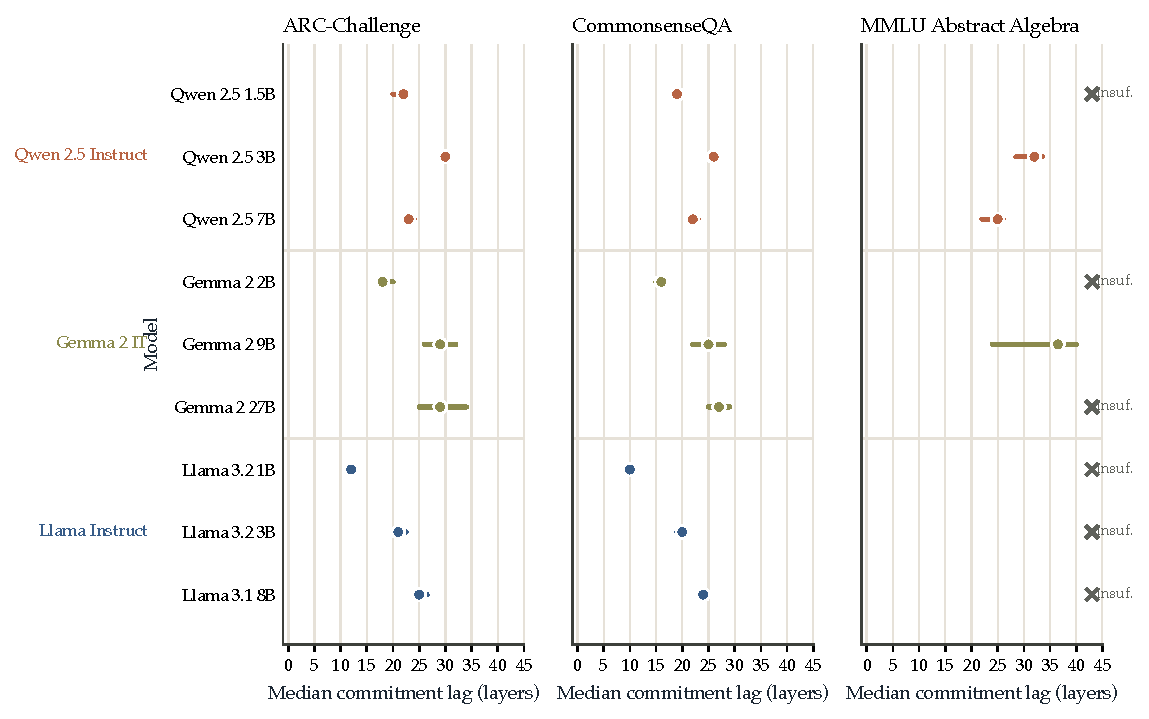
\includegraphics[width=\textwidth]{figure2_primary_forest_plot.pdf}
\caption{\textbf{Every evaluable ARC-Challenge and CommonsenseQA cell is positive under the preregistered primary rule.} Each point is the cell-level median commitment lag $\Delta_{\mathrm{margin}}$ in raw layer units for the primary analysis path, and each horizontal interval is a grouped-bootstrap 95\% confidence interval. All evaluated ARC-Challenge and CommonsenseQA cells are positive. The MMLU abstract-algebra slice contributes several \emph{insufficient n} cells because the slice itself contains only 11 questions and the preregistration requires at least ten valid examples per model-dataset cell.}
\label{fig:forest}
\end{figure*}

Figure~\ref{fig:forest} and Table~\ref{tab:primary-summary} translate the pooled picture into the preregistered cell-level decision rule. All \ArcCsqaPositiveCells{} evaluable ARC-Challenge and CommonsenseQA cells are positive, and there are no evaluated negatives. Across all three datasets, \OverallPrimaryPositiveCells{} cells are positive and \OverallPrimaryInsufficientCells{} are insufficient. Within MMLU specifically, \MmluPositiveCells{} cells are positive and \MmluInsufficientCells{} are insufficient. That is what we would expect from a very small benchmark slice under a minimum-valid-example rule.

\begin{table}[t]
\centering
\small
\begin{tabular}{@{}lccc@{}}
\toprule
Dataset & Positive & Evaluable & Insufficient \\
\midrule
ARC-Challenge & 9 & 9 & 0 \\
CommonsenseQA & 9 & 9 & 0 \\
MMLU Abstract Algebra & 3 & 3 & 6 \\
All datasets & 21 & 21 & 6 \\
\bottomrule
\end{tabular}

\caption{\textbf{Primary-rule summary by dataset.} ARC-Challenge and CommonsenseQA are positive in every evaluable model-dataset cell. The only non-positive outcomes are \emph{insufficient n} cells from the small MMLU abstract algebra slice.}
\label{tab:primary-summary}
\end{table}

The family-level summaries tell the same story. Qwen contributes eight positive primary cells, Gemma contributes seven, and Llama contributes six. In every family, the missing positives are insufficient MMLU cells rather than evaluated negatives. So the result is broad across the chosen instruct-model panel, even though the exact lag size still varies with model depth and dataset difficulty.

\FloatBarrier

\section{Controls and robustness}

The controls change only one thing: the exact string scored after \texttt{"Final answer: "}. Figure~\ref{fig:controls} shows why that matters. Under identity ordering, the primary exact-option readout yields a \SemanticIdentityValidRate{} valid-rate for $\Delta_{\mathrm{margin}}$. If we keep the prompt fixed but score the literal continuation \texttt{"The answer is \{option\}"} instead, that valid-rate falls to \TemplatedIdentityValidRate{}. If we score only the answer letter, it rises to \LetterIdentityValidRate{}.

\begin{figure}[t]
\centering
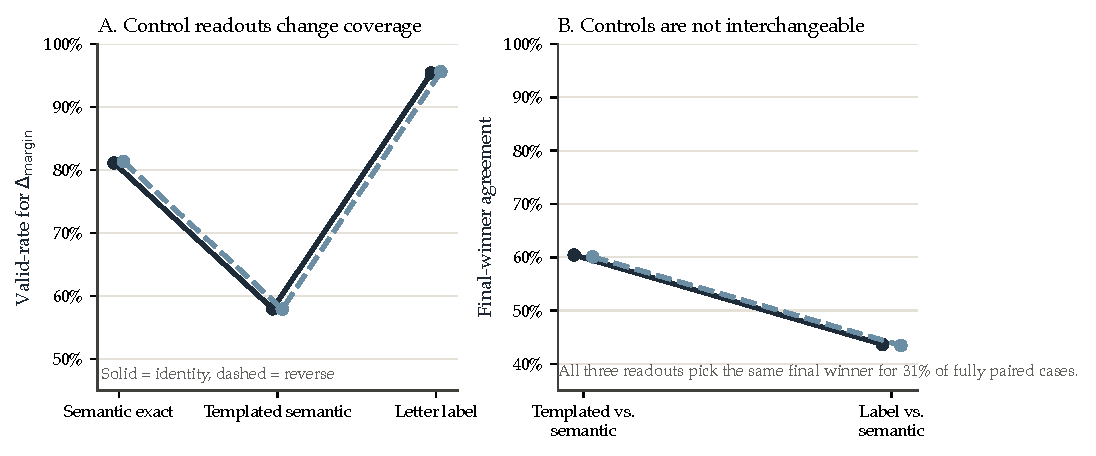
\includegraphics[width=\columnwidth]{figure3_control_readout_comparison.pdf}
\caption{\textbf{Changing only the answer format changes the measurement.} Panel A shows how often $\Delta_{\mathrm{margin}}$ is defined for each readout. Panel B shows how often the two control readouts pick the same final winner as the semantic-exact primary readout on fully paired cases. Identity and reverse order behave similarly, which is good. The answer-format controls do not, which is exactly why they must stay controls rather than replacing the main semantic path.}
\label{fig:controls}
\end{figure}

The readouts also disagree on which answer the model prefers at the end. In fully paired identity cases, the templated control agrees with the exact-option path on only \TemplatedAgreementIdentity{} of cases, the letter-label control agrees on only \LetterAgreementIdentity{}, and all three readouts agree on just \AllSameReadoutRate{} of cases. This does not weaken the main result. It tells us something important about measurement: scoring \texttt{"A"} is not the same experiment as scoring \texttt{"photosynthesis"}. The controls are useful because they reveal answer-format effects. They are not suitable replacements for the main semantic readout.

The answer-order control tells a different story. In Figure~\ref{fig:controls}, the identity and reverse traces are nearly on top of each other. That is reassuring because it suggests the main effect is not coming from one arbitrary option order. The report-only robustness summaries also line up with the primary rule. The secondary criterion yields the same positive-versus-insufficient pattern as the primary rule (\OverallSecondaryPositiveCells{} positive, \OverallSecondaryInsufficientCells{} insufficient), and the gold-answer sensitivity analysis is positive on all \GoldArcCsqaPositiveCells{} evaluable ARC-Challenge and CommonsenseQA cells while remaining underpowered on the MMLU slice (\GoldMmluInsufficientCells{} insufficient cells).

Finally, the QC path is designed to surface problems, not hide them. The released audit bundle logs \TokenCollisionCount{} tokenization collisions and \DuplicateOptionCount{} duplicate-option examples instead of silently dropping them, while the merged run itself still has zero failure rows and zero unpaired rows. The point is not to make the result look tidy. The point is to show that the result still holds when we keep the pipeline honest about edge cases.

\FloatBarrier

\section{Interpretation and limits}

Figure~\ref{fig:exemplars} shows what the aggregate result looks like in individual cases. Each panel plots the winner-minus-runner contrast for one semantic-exact identity example. The details differ by family and prompt, but the same broad pattern appears again and again: the eventual answer becomes plausible early, while stable commitment arrives much later and can be preceded by hesitation or reversals.

\begin{figure*}[t]
\centering
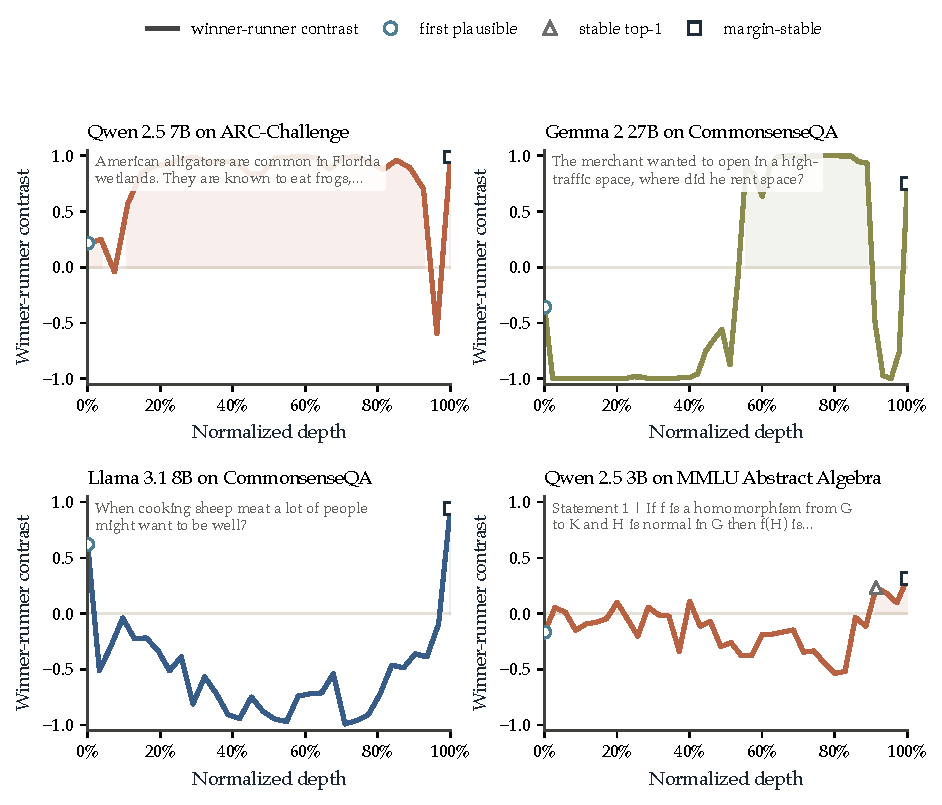
\includegraphics[width=\textwidth]{figure4_prompt_level_exemplars.pdf}
\caption{\textbf{Prompt-level trajectories show the same pattern as the pooled figures.} Each panel plots the winner-minus-runner contrast across normalized depth for one semantic-exact identity example. The circular marker shows when the eventual answer first enters the plausible set, the triangular marker shows when it becomes stable top-1, and the square marker shows when it becomes margin-stably committed. The exact shapes vary, but the same left-to-right separation between plausibility and commitment appears at the single-case level.}
\label{fig:exemplars}
\end{figure*}

These measurements still need to be interpreted carefully. We are not claiming that the model literally stores a human-like list of hypotheses, and we are not claiming that these curves identify a full causal circuit. Our claim is narrower. Under this prompting and scoring setup, the eventual answer often enters the plausible-answer set before it becomes stably isolated from the runner-up.

The empirical scope is also narrow in three practical ways. First, the paper uses a 1{,}000-example slice rather than the full benchmark splits. Second, the panel contains only instruction-tuned open-weight models, so the claim should not be generalized to base models or closed systems. Third, MMLU abstract algebra contributes only \MmluPromptCount{} questions because that entire validation slice is tiny in this setup. That is why most of its model-dataset cells are underpowered under the preregistered minimum-valid-example rule.

Those limits matter, but they do not erase the signal. The early-plausibility/late-commitment pattern appears in the pooled depth curves, in every evaluable ARC-Challenge and CommonsenseQA cell, and in the prompt-level trajectories. The controls matter here too. They show that small changes in answer format can change coverage and final winners, which is exactly why the paper keeps exact option-text scoring as the main path.

\FloatBarrier

\section{Conclusion}

The paper's claim is simple and deliberately scoped. In the setting we study, instruction-tuned models often know which answers are still possible before they have fully settled on the one they will finally say. We show that pattern by ending each prompt with \texttt{"Final answer: "} and tracking how the scores of exact answer continuations change across model depth.

The evidence is consistent across levels of analysis. The flagship pooled curves show a large gap between plausibility and commitment. Every evaluable ARC-Challenge and CommonsenseQA model-dataset cell is positive under the preregistered primary rule. The prompt-level examples show the same separation in concrete trajectories. The answer-format controls matter because they show that this result is not automatic: changing the continuation string can change both coverage and winners.

The result does not yet explain why the gap appears, and it should not be overgeneralized beyond this panel and benchmark slice. But it does support a useful empirical distinction for future work. The moment when a model finally says an answer can come much later than the moment when that answer first becomes one of the answers the model already treats as plausible.


\bibliographystyle{colm2026_conference}
\bibliography{references}

\onecolumn
\appendix
\section{Supplementary material}

\subsection{Reproducibility statement}

This manuscript is generated from a single merged run, \texttt{\MergedRunId}, with run-scoped manifests, QC summaries, bootstrap outputs, and figure/table provenance checked into the paper workspace. All numeric claims in the paper are generated from those artifacts rather than entered by hand. The merged run contains \PreparedExampleCount{} prepared prompts, \ScoreRowCount{} scored units, \MetricRowCount{} metric rows, and \TokenAuditCount{} token audits.

\subsection*{Ethics statement}

This study analyzes public benchmark questions using open-weight language models and does not involve human subjects, personal data, or deployment to end users. The main risk is analytical overclaiming: layerwise statistics can be mistaken for a complete mechanistic explanation when they are only an operational measurement. We mitigate that risk by keeping the claim narrow, preregistering the primary rule, preserving anomaly logs, and explicitly reporting the underpowered status of the MMLU slice.

\subsection*{AI-use disclosure}

AI-use disclosure. The authors used AI-assisted tools during the project lifecycle: ChatGPT for brainstorming and experimental design iteration, Codex for implementation assistance, and Claude Opus for drafting and formatting portions of the manuscript and LaTeX source. All scientific decisions, experiments, analyses, code review, result verification, and final manuscript editing were performed and approved by the human authors, who take full responsibility for the paper’s contents.

\subsection{Model registry}

\begin{center}
\small
\begin{tabularx}{\linewidth}{@{}lllXX@{}}
\toprule
Family & Model & Size & Repository & Revision prefix \\
\midrule
Qwen 2.5 Instruct & Qwen 2.5 1.5B & 1.5b & Qwen2.5-1.5B-Instruct & \texttt{989aa7980e4c} \\
Qwen 2.5 Instruct & Qwen 2.5 3B & 3b & Qwen2.5-3B-Instruct & \texttt{aa8e72537993} \\
Qwen 2.5 Instruct & Qwen 2.5 7B & 7b & Qwen2.5-7B-Instruct & \texttt{a09a35458c70} \\
Gemma 2 IT & Gemma 2 2B & 2b & gemma-2-2b-it & \texttt{299a8560bedf} \\
Gemma 2 IT & Gemma 2 9B & 9b & gemma-2-9b-it & \texttt{11c9b309abf7} \\
Gemma 2 IT & Gemma 2 27B & 27b & gemma-2-27b-it & \texttt{aaf20e6b9f4c} \\
Llama Instruct & Llama 3.2 1B & 1b & Llama-3.2-1B-Instruct & \texttt{9213176726f5} \\
Llama Instruct & Llama 3.2 3B & 3b & Llama-3.2-3B-Instruct & \texttt{0cb88a4f764b} \\
Llama Instruct & Llama 3.1 8B & 8b & Meta-Llama-3.1-8B-Instruct & \texttt{0e9e39f249a1} \\
\bottomrule
\end{tabularx}

\captionof{table}{\textbf{Model registry used in the paper.} Short repository names and 12-character revision prefixes are shown for readability; the full pinned revision hashes are preserved in the released provenance manifest.}
\label{tab:model-registry}
\end{center}

\subsection{Full primary positivity table}

\begin{center}
\scriptsize
\begin{tabularx}{\textwidth}{@{}llcccc@{}}
\toprule
Dataset & Model & Valid / total & Median lag & 95\% CI & Primary decision \\
\midrule
ARC-Challenge & Qwen 2.5 1.5B & 109/195 & 22 & [20, 23] & positive \\
ARC-Challenge & Qwen 2.5 3B & 143/195 & 30 & [29, 31] & positive \\
ARC-Challenge & Qwen 2.5 7B & 163/195 & 23 & [22, 24] & positive \\
ARC-Challenge & Gemma 2 2B & 117/195 & 18 & [17, 20] & positive \\
ARC-Challenge & Gemma 2 9B & 132/195 & 29 & [26, 32] & positive \\
ARC-Challenge & Gemma 2 27B & 135/195 & 29 & [25, 34] & positive \\
ARC-Challenge & Llama 3.2 1B & 79/195 & 12 & [11, 13] & positive \\
ARC-Challenge & Llama 3.2 3B & 104/195 & 21 & [20, 22] & positive \\
ARC-Challenge & Llama 3.1 8B & 112/195 & 25 & [24, 26] & positive \\
CommonsenseQA & Qwen 2.5 1.5B & 677/794 & 19 & [18, 20] & positive \\
CommonsenseQA & Qwen 2.5 3B & 706/794 & 26 & [25, 26] & positive \\
CommonsenseQA & Qwen 2.5 7B & 718/794 & 22 & [22, 23] & positive \\
CommonsenseQA & Gemma 2 2B & 693/794 & 16 & [15, 17] & positive \\
CommonsenseQA & Gemma 2 9B & 702/794 & 25 & [22, 28] & positive \\
CommonsenseQA & Gemma 2 27B & 706/794 & 27 & [25, 29] & positive \\
CommonsenseQA & Llama 3.2 1B & 625/794 & 10 & [9, 10] & positive \\
CommonsenseQA & Llama 3.2 3B & 672/794 & 20 & [19, 21] & positive \\
CommonsenseQA & Llama 3.1 8B & 649/794 & 24 & [23, 25] & positive \\
MMLU Abstract Algebra & Qwen 2.5 1.5B & 7/11 & -- & -- & insufficient n \\
MMLU Abstract Algebra & Qwen 2.5 3B & 10/11 & 32 & [28, 33] & positive \\
MMLU Abstract Algebra & Qwen 2.5 7B & 10/11 & 25 & [22, 26] & positive \\
MMLU Abstract Algebra & Gemma 2 2B & 7/11 & -- & -- & insufficient n \\
MMLU Abstract Algebra & Gemma 2 9B & 10/11 & 36 & [24, 40] & positive \\
MMLU Abstract Algebra & Gemma 2 27B & 7/11 & -- & -- & insufficient n \\
MMLU Abstract Algebra & Llama 3.2 1B & 4/11 & -- & -- & insufficient n \\
MMLU Abstract Algebra & Llama 3.2 3B & 2/11 & -- & -- & insufficient n \\
MMLU Abstract Algebra & Llama 3.1 8B & 2/11 & -- & -- & insufficient n \\
\bottomrule
\end{tabularx}

\captionof{table}{\textbf{Full cell-level primary-rule results.} The primary decision is evaluated separately for each model-dataset cell on the semantic-exact identity path.}
\label{tab:full-positivity}
\end{center}

\subsection{Selection and QC details}

\begin{center}
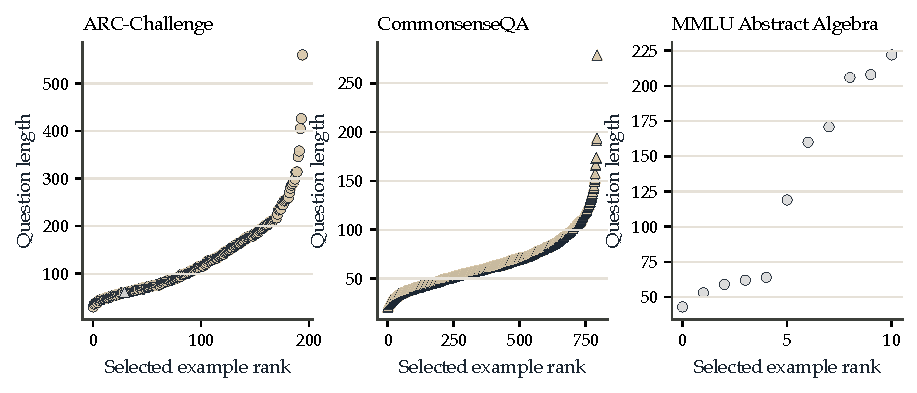
\includegraphics[width=\linewidth]{appendix_selection_profile.pdf}
\captionof{figure}{\textbf{The paper slice spans a wide range of selected prompt lengths.} The figure shows the selected-example question-length profile for each dataset together with the chosen option-count markers. MMLU is exhausted because the abstract-algebra validation slice contains only \MmluPromptCount{} prompts.}
\label{fig:selection}
\end{center}

\begin{center}
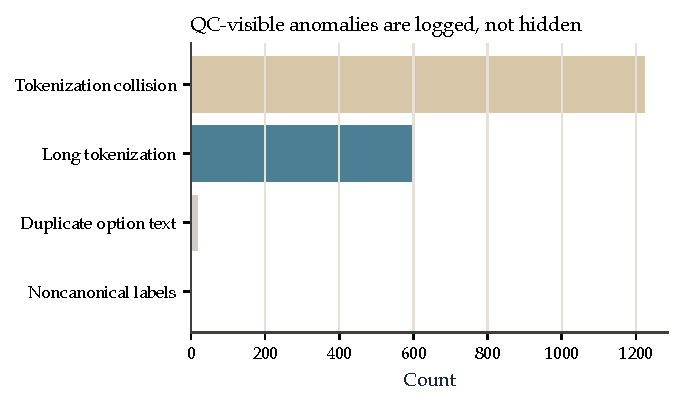
\includegraphics[width=\columnwidth]{appendix_qc_anomalies.pdf}
\captionof{figure}{\textbf{QC-visible anomalies are logged rather than hidden.} These counts come directly from the merged run's QC summary. They motivate caution, but they do not arise from silent exclusion or failed pairing.}
\label{fig:qc}
\end{center}

\begin{center}
\small
\begin{tabular}{@{}lc@{}}
\toprule
QC item & Count \\
\midrule
Prepared examples & 1000 \\
Token audits & 258876 \\
Tokenization collisions & 1224 \\
Suspiciously long option tokenizations & 594 \\
Duplicate option text & 17 \\
Noncanonical option labels & 2 \\
Unpaired rows & 0 \\
Failure rows & 0 \\
\bottomrule
\end{tabular}

\captionof{table}{\textbf{QC summary for the merged run.} The run completes with zero failure rows and zero unpaired rows while still surfacing tokenization and option-surface anomalies.}
\label{tab:qc-summary}
\end{center}

\begin{center}
\small
\begin{tabularx}{\linewidth}{@{}lXl@{}}
\toprule
Readout & Continuation surface & Normalization \\
\midrule
semantic\_exact & Exact option text after \texttt{"Final answer:"}, e.g. \texttt{"photosynthesis"} & Mean log-probability \\
templated\_semantic & Literal continuation \texttt{"The answer is \{option\_text\}"} & Mean log-probability \\
letter\_label & Bare answer letter after \texttt{"Final answer:"}, e.g. \texttt{"A"} & Mean log-probability \\
\bottomrule
\end{tabularx}

\captionof{table}{\textbf{Readout definitions used in the paper.} The controls intentionally differ in continuation surface while keeping the rest of the setup fixed.}
\label{tab:readout-defs}
\end{center}


\end{document}
